\subsection{Overall Description}
\begin{description}
	\item[Dimensions] 57 mm ${\times}$ 57 mm ${\times}$ 57 mm
	\item[Weight]	100 g
	\item[Material] Hard plastic
	\item[Appearance] Black; individual facelets are coated by a brightly coloured sticker to differentiate the faces.
\end{description}
\subsection{Description of Parts}
	\subsubsection{Central Core}\label{part:cross}
		The central 3D cross holds the cube together. It has a yoke(see \figref{yoke}), along which are attached the six centre facelets(see \figref{centre}). The resultant part is shown in \figref{cross}.
		\begin{figure}[h]
			\centering
			\begin{subfigure}[b]{0.3\textwidth}
				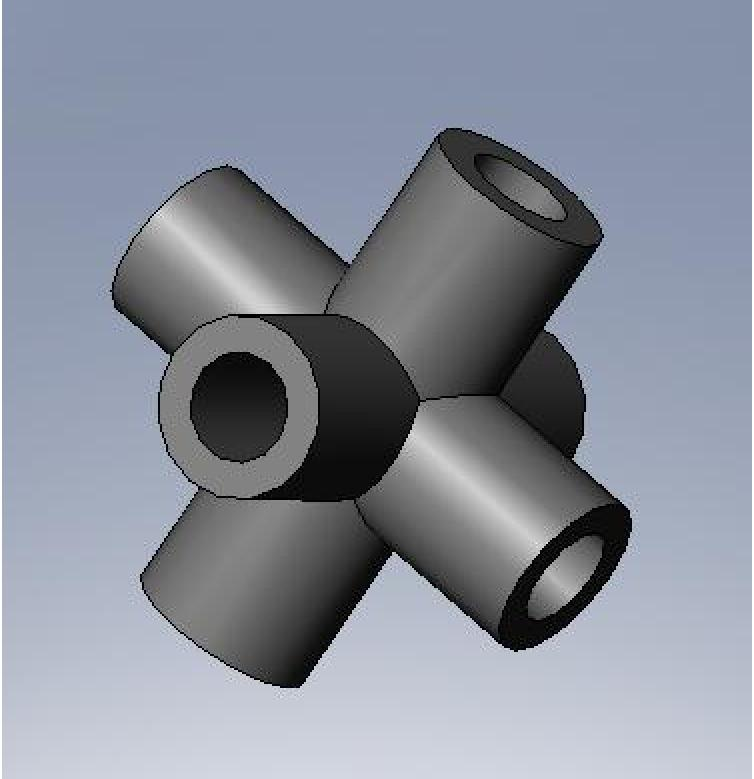
\includegraphics[width=\textwidth]{yoke.jpg}
				\caption{Yoke}\label{fig:yoke}
			\end{subfigure}
			\begin{subfigure}[b]{0.3\textwidth}
				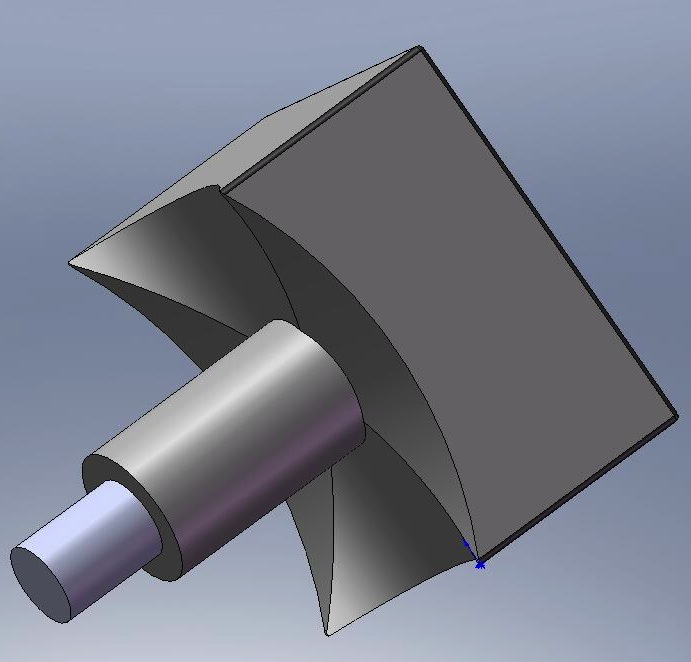
\includegraphics[width=\textwidth]{center.jpg}
				\caption{Centre facelet}\label{fig:centre}
			\end{subfigure}
			\begin{subfigure}[b]{0.3\textwidth}
				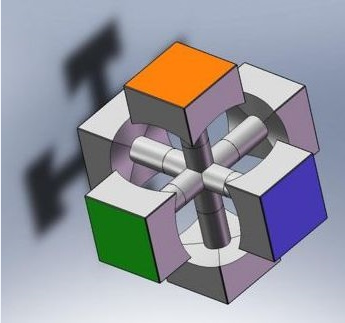
\includegraphics[width=\textwidth]{cross.png}
				\caption{Cross}\label{fig:cross}
			\end{subfigure}
			\caption{Core}
		\end{figure}
	\subsubsection{Exterior Facelets}
		Surrounding the cross described in~\ref{part:cross} are edge(\figref{edge}) and corner(\figref{corner}) cubelets, with two and three facelets respectively. They feature extrusions that lock them to the core, while still allowing them to be manipulated easily.
		\begin{figure}[h]
			\centering
			\begin{subfigure}[b]{0.4\textwidth}
				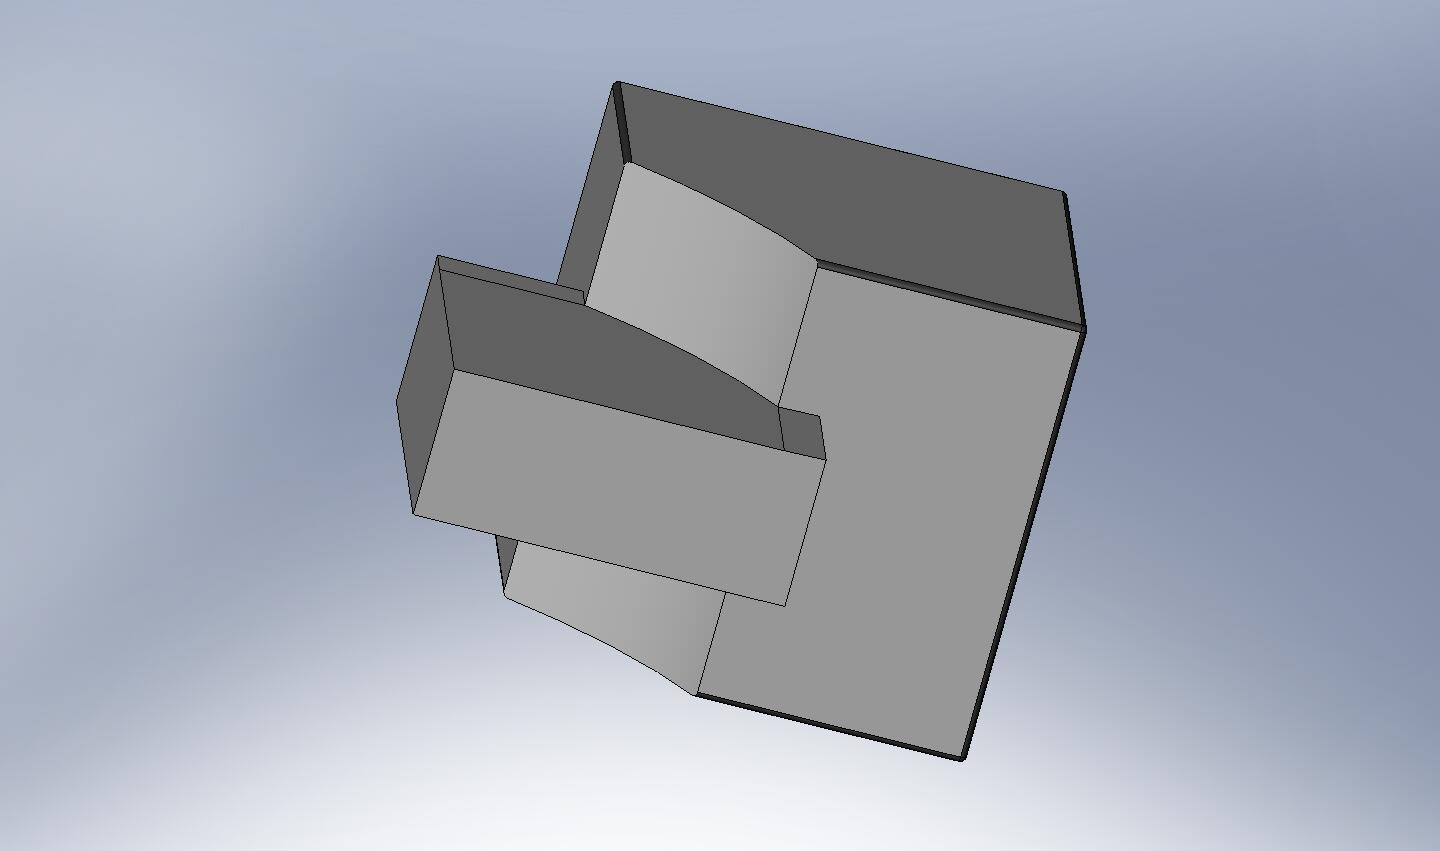
\includegraphics[width=\textwidth]{edge.jpg}
				\caption{Edge}\label{fig:edge}
			\end{subfigure}
			\begin{subfigure}[b]{0.4\textwidth}
				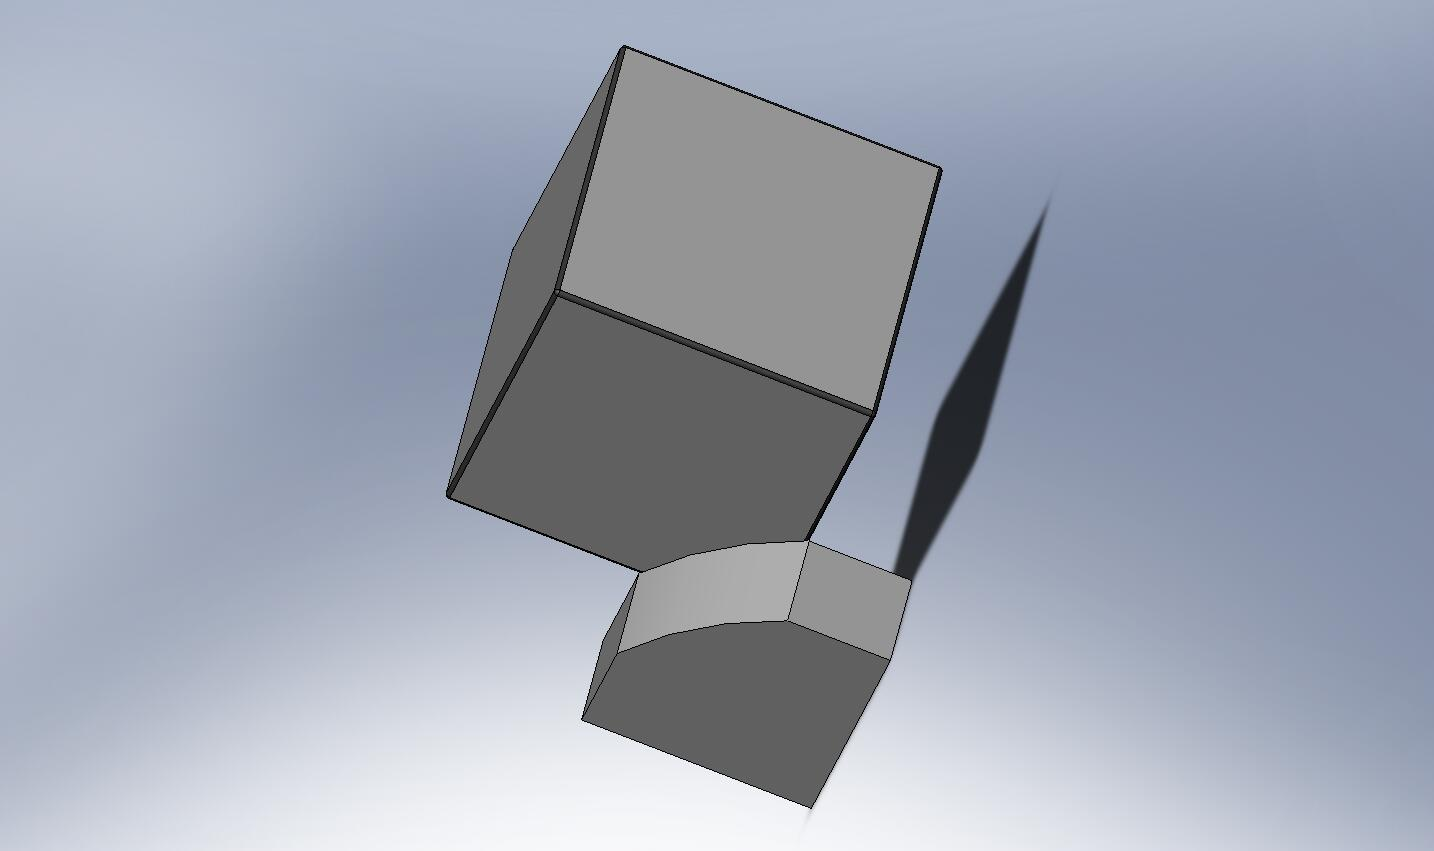
\includegraphics[width=\textwidth]{corner.jpg}
				\caption{Corner}\label{fig:corner}
			\end{subfigure}
			\caption{Exterior facelets}
		\end{figure}